% !TEX program = xelatex
% !TEX root = main-submission.tex
% ---------------------------------------------------------------------
% Anonymity.  AAMAS 2027 reviews double-blind, so \blindtrue switches on
% the aamas class's anonymous option and leaves authors.tex unread: the
% PDF shows "Anonymous Author(s)", the running head shows "Anon.", and
% the XMP/PDF author metadata is anonymized as well.  Set \blindfalse
% for the camera-ready build.
% ---------------------------------------------------------------------
\newif\ifblind
\blindtrue
\ifblind\PassOptionsToClass{anonymous=true}{aamas}\fi
\documentclass[sigconf]{aamas}
\usepackage{amsmath}
\usepackage{balance}
\usepackage{algorithm}
\usepackage{algpseudocode}

% The class sets neither \tolerance nor \emergencystretch, so in this narrow
% two-column measure TeX frequently finds no feasible break sequence and lets
% words run past the right margin.  Emergency stretch is only used in the
% final pass, once the normal pass has already failed: it costs nothing on
% lines that fit and leaves geometry, fonts, and spacing parameters untouched.
\setlength{\emergencystretch}{1em}

% =====================================================================
% Reporting-name map.  Paper names (left) -> internal experiment codes
% (right), so every number below stays traceable to the result bundle.
%   No-filter         = B0            Similarity-grouping = C (main)
%   Relevance         = B1            NLI-grouping        = A
%   Dedup             = B2            Hard-cut            = S0
%   NLI-consistency   = B4            Floor-preserving    = S2
%   TrustRAG-adapt    = B5            ConGuard-4f         = C4
%   Per-doc-LOO       = B6            ConGuard-3f         = C3-feature
%   ConGuard + Floor  = C--G1         ConGuard-3m         = C3-mechanism
%   ConGuard + Cut    = C--G0         ConGuard-hgate      = C4-hgate
%   NLI-group + Floor = A--G1         NLI-group + Cut     = A--G0
% =====================================================================

% Copyright block from the AAMAS 2027 template; class and layout unchanged.
\makeatletter
\gdef\@copyrightpermission{
  \begin{minipage}{0.2\columnwidth}
   \href{https://creativecommons.org/licenses/by/4.0/}{
\includegraphics[width=0.90\textwidth]{by}}
  \end{minipage}\hfill
  \begin{minipage}{0.8\columnwidth}
   \href{https://creativecommons.org/licenses/by/4.0/}{This work is licensed under a Creative Commons Attribution International 4.0 License.}
  \end{minipage}
  \vspace{5pt}
}
\makeatother
\setcopyright{ifaamas}
\acmConference[AAMAS 2027]{Proc.\@ of the 26th International Conference
on Autonomous Agents and Multiagent Systems (AAMAS 2027)}{3--7 May 2027}{Hanoi, Vietnam}{M.~Baldoni, F.~Fang, W.~Yeoh, N.~Yorke-Smith (eds.)}
\copyrightyear{2027}
\acmYear{2027}
\acmDOI{}
\acmISBN{}
% Fill in the actual identifier after registering the abstract on OpenReview.
\InputIfFileExists{submission-id.tex}{}{\acmSubmissionID{}}
\submissionType{Research Paper Track}
\title[RAG-ConGuard: Coalition-Level Evidence Filtering]{RAG-ConGuard: Coalition-Level Evidence Filtering and Safety--Availability Trade-offs in Poisoned RAG}
% Author block: skipped while \blindtrue.  With no \author command the
% class prints its own "Anonymous Author(s)" placeholder, which is what
% the submission should show.
\ifblind\else% !TEX root = main-submission.tex
% =====================================================================
% Author block -- real names, affiliations, and contact details.
%
% This file is NOT read by the double-blind submission build.  main.tex
% sets \blindtrue, which turns on the aamas class's anonymous option and
% skips this file, so the submission PDF shows "Anonymous Author(s)" and
% carries no author metadata.
%
% Camera-ready: set \blindfalse in main.tex; this block is then included
% and the class option is dropped automatically.
% =====================================================================
\author{Jinsong Yang}
\email{yangjinsong@gs.zzu.edu.cn}
\orcid{0009-0009-3038-3667}
\affiliation{%
  \institution{Zhengzhou University}
  \city{Zhengzhou}
  \state{Henan}
  \country{China}}

\author{Enhao Zhang}
\email{zhangeh@zzu.edu.cn} % TODO: confirm actual email.
\affiliation{%
  \institution{Zhengzhou University}
  \city{Zhengzhou}
  \state{Henan}
  \country{China}}

\author{Zhihua Wang}
\authornote{Corresponding author.}
\email{zhwang@zzu.edu.cn} % TODO: confirm actual corresponding-author email.
\affiliation{%
  \institution{Zhengzhou University}
  \city{Zhengzhou}
  \state{Henan}
  \country{China}}

\renewcommand{\shortauthors}{Yang et al.}
\fi

\begin{abstract}
Knowledge-grounded agents answer from retrieved passages, which gives an attacker who can write into the corpus an indirect influence channel: promoting a chosen answer by repeating it across several passages. Because such repetition survives the removal of any single passage, filters that score passages in isolation leave this attack largely intact---on our evaluation, relevance filtering changes no attack outcome, and NLI-consistency filtering raises attack success from 83.3\% to 86.7\% by deleting passages the generator relied on. To this end, we present RAG-ConGuard, an inference-time evidence filter that groups semantically related passages into \emph{evidence coalitions}, summarizes their signed relations in a compact graph, and predicts risk at the group level, with two context selectors that expose the trade-off between removing suspicious evidence and retaining a nonempty context. On a 60-query attacked evaluation spanning three question-answering datasets, the availability-oriented configuration reduces attack success from 83.3\% to 48.3\% at a 10.0\% refusal rate (6 of 60 queries, up from 1), and an aggressive configuration reaches 18.3\% attack success at 45.0\% refusal; a TrustRAG adaptation attains 15.0\% at 48.3\%, so the measured points do not establish dominance over that baseline. Four-variant, three-seed ablations show no aggregate benefit from the auxiliary graph-support \emph{Impact} feature at the availability point, and generation-distribution probes, including complete evidence removal, do not validate it as a proxy for generation effects---indicating that counterfactual graph support should not be substituted for a measured generator response. Clean-answer scores are unchanged on 300 gold-available HotpotQA queries, while clean refusal rises on MS MARCO. The results characterize coalition-level filtering as a configurable safety--availability trade-off; generalization is measured on a single development-exposed attack construction, and no causal attribution is claimed.
\end{abstract}
\keywords{retrieval-augmented generation, knowledge poisoning, evidence filtering, trustworthy agents, abstention}
\ccsdesc[500]{Security and privacy}
\ccsdesc[300]{Computing methodologies~Natural language generation}

\begin{document}
\maketitle

\section{Introduction}
Retrieval-augmented generation (RAG) supplies language models with external evidence for knowledge-intensive tasks~\cite{rag}, and knowledge-grounded agents increasingly depend on that evidence when they answer, plan, and act. This dependence creates an indirect influence channel: an attacker who can insert text into the corpus can shape what the agent reads before it reasons. Targeted knowledge-corruption attacks exploit precisely this channel, promoting an incorrect answer through retrieved text rather than through the model's weights~\cite{poisonedrag}. The relevant intervention point is therefore not only the agent's final response but also the evidence it is permitted to consume, and controlling that intake is a defensive capability in its own right.

A single decisive passage is not what makes these attacks work. An attacker can distribute the same misleading proposition across several retrieved passages, so that the claim survives the deletion of any individual document. Repetition of this kind also arises among legitimate passages, and group size plus internal agreement cannot by itself establish malicious coordination, since several agreeing documents need not represent independent sources. A filter must therefore remove suspicious groups while retaining enough evidence for the generator to answer at all.

Filtering passages one at a time is insufficient here, and our measurements show how sharply. A relevance filter changes no attack outcome relative to no filtering whatsoever: both conditions produce 50 successful attacks out of 60 queries. An NLI-consistency filter, which deletes passages that disagree with the retrieved majority, is worse still---it raises attack success from 83.3\% to 86.7\% by discarding the passages the generator needed. Both filters evaluate one passage at a time, whereas the attacker controls several at once.

To address this, we present RAG-ConGuard, an inference-time evidence filter that scores evidence jointly rather than individually. RAG-ConGuard extracts one short excerpt per passage, groups excerpts by semantic similarity subject to a pairwise contradiction check, and computes structural features from a signed natural-language-inference (NLI) graph. A small supervised classifier assigns a risk score to each eligible group, which we term an \emph{evidence coalition}. One selector then removes every coalition above a risk threshold, while another preserves a minimum number of passages. Throughout, a coalition is a group of evidence items, not a collection of autonomous agents or a game-theoretic solution concept.

Two questions guide the evaluation, and we keep them separate because a filter that works does not thereby validate each of its inputs. The first is whether the grouping and selection pipeline offers a useful operating point. The second is what explains its behavior. In particular, an auxiliary \emph{Impact} score measures how graph-derived evidence support changes when a coalition is removed. This is a counterfactual calculation on a deterministic graph operator, and its relation to the generator's behavior must be measured separately rather than assumed.

Filtering reduces attack success, and it also costs availability. The retained-context point still permits 29 attacks among 60 queries; the aggressive point permits 11 attacks but refuses 27 queries; the TrustRAG adaptation permits nine attacks and refuses 29. These outcomes support configurable filtering without establishing superiority over that baseline.

Overall, our contributions are threefold.
\begin{itemize}
\item We propose RAG-ConGuard, an inference-time coalition-level filter that combines semantic grouping, signed graph features, and policies for context retention, with a clear separation between risk estimation and evidence selection.
\item We measure attack success, answer match, and refusal on three question-answering datasets, reporting two operating points, generator transfer, and a partially labeled clean evaluation.
\item We separate Impact's role as a classifier input from its role in the eligibility rule, and compare graph-support changes against generation-distribution probes and available same-size deletion controls, finding no aggregate benefit at the availability point.
\end{itemize}
Our experiments isolate evidence use in single-turn question answering, which is the point at which a knowledge-grounded agent consumes retrieved text; planning, tool use, multiagent coordination, and long-horizon task completion are not evaluated. The attacked evaluation queries were examined during development, so the results are exploratory rather than an independent confirmation of generalization.

\section{Related Work}
\paragraph{Corpus poisoning and service availability.}
PoisonedRAG formulates targeted knowledge corruption through a small number of injected passages~\cite{poisonedrag}. We adopt the corresponding target-answer threat model with a project-specific synthetic attack construction, and we do not claim to reproduce every attack optimization in that work. SafeRAG broadens evaluation to several security failure modes, including conflicting evidence and denial of service~\cite{saferag}. These distinctions motivate reporting refusal separately from target-answer success, because a defense can reduce the latter while making the system less useful. Our experiment covers targeted answer poisoning rather than the full SafeRAG benchmark.

\paragraph{Filtering untrusted evidence.}
TrustRAG uses clustering followed by a self-assessment process to distinguish malicious information and to reconcile retrieved with internal knowledge~\cite{trustrag}. ShieldRAG defends against untrusted knowledge using adversarial generation and evaluation components~\cite{shieldrag}. Our method differs in learning a small classifier over group features and applying an explicit context-retention policy; this difference does not imply that existing defenses ignore context relations. Our TrustRAG-adapt comparison is an adaptation of TrustRAG to the project pipeline, and its measured operating point is not a refusal-matched comparison against the original system.

\paragraph{Evidence representation and attribution.}
The retriever uses dense embeddings from the BGE family~\cite{bge} alongside sparse retrieval, and the datasets are drawn from retrieval-oriented question-answering resources~\cite{beir}. NLI relations provide an approximate signed structure over excerpts~\cite{nlimodel}, and such relations are not factuality certificates or measurements of source independence. Likewise, deleting nodes from a support graph and deleting passages from a generator's context are different interventions, so we use teacher-forced distribution comparisons to examine their association and stop short of identifying a causal effect on answer correctness or autonomous behavior.

\paragraph{Positioning.}
Across these lines of work, defenses are evaluated mainly on whether they suppress a targeted answer, and the availability cost of suppression is reported less consistently. Our contribution is complementary to that literature: we treat the removal decision itself as the object of study, score evidence at the group level, and report attack success, answer match, and refusal jointly so that the operating trade-off is visible rather than implied.

\section{Problem Setup and Threat Model}
Let $q$ be a query, $\mathcal{K}$ a corpus, and $D=(d_1,\ldots,d_n)$ the ranked retrieved context. A generator $f_\theta$ produces an answer from $q$ and a selected subsequence $D'\subseteq D$. The attacker inserts a set $P$ of passages into $\mathcal{K}$ to induce a chosen incorrect answer $y^{\mathrm{adv}}_q$. The attacker controls inserted text but not the defender's model weights, system prompt, or scoring labels. The evaluated budget is five injected passages per target query, and retrieval returns $n=5$ passages. The defender observes the query and the retrieved text; it does not use either the correct answer or $y^{\mathrm{adv}}_q$ to construct runtime features.

We examine three outcomes: production of the target answer, production of a reference-matching answer, and refusal. All rates use the full evaluated query set as their denominator. Refusal is a loss of availability in this task even when it prevents an attack, and a non-refusal is not automatically a correct answer. A document-retention floor constrains evidence deletion only; it guarantees neither correctness nor a bound on generator refusal.

The attacker's passages may form a semantically coherent cluster, but we assume no trusted provenance signal. Our use of ``coalition'' therefore describes this measurable grouping rather than establishing common authorship, independent corroboration, or actual cooperation between document sources. The reported attacks are fixed constructions, and detector-aware adaptive robustness lies outside the validated experimental scope.

\section{Coalition-Level Evidence Filtering}
\label{sec:method}
RAG-ConGuard operates in three stages, and we separate them deliberately because they carry different evidential weight. It first builds a compact representation of the retrieved context from excerpts and signed NLI relations, then derives structural features from a graph-support operator, and finally scores coalitions with a small classifier whose eligible groups are passed to one of two context selectors. The following subsections detail these stages in turn.

\subsection{Excerpts, Relations, and Grouping}
Each retrieved passage contributes its leading 220 characters as one excerpt $c_i$. This truncation does not extract claims based on the query and can omit relevant text. BGE embeddings $e_i$ represent these excerpts, and a cross-encoder NLI model assigns support, contradiction, or neutral relations to directed excerpt pairs. The resulting graph is $G=(V,E^+,E^-)$, with neutral relations discarded. The pipeline also supports a numerical-conflict check; the reported configuration uses NLI-based relation extraction rather than an LLM judge.

Grouping and signed feature extraction use distinct relations. The semantic grouping graph joins $i$ and $j$ when $\cos(e_i,e_j)\geq0.85$ and the pair is not marked contradictory, and its connected components are coalition candidates. They are not simply positive-NLI connected components, because transitive connectivity can still place an indirectly connected contradictory pair in the same component; a coalition therefore need not be globally consistent. The positive-edge grouping variant appears as NLI-grouping in the experiments.

For a coalition $C$ of size $m\geq2$, define $U^+$ and $U^-$ as the deduplicated unordered versions of $E^+$ and $E^-$. Two structural features are
\begin{align}
h(C)&=\frac{|\{\{i,j\}\in U^+:i,j\in C\}|}{\binom{m}{2}},\\
r(C)&=\frac{|\{\{i,j\}\in U^-:|\{i,j\}\cap C|=1\}|}{m}.
\end{align}
The cohesion $h$ counts internal support, and $r$ counts crossing contradictions per member. In particular, $r$ is not the probability of refutation or of support for a competing answer. Deduplicating edges here prevents double counting directed NLI pairs, whereas the support operator below retains directed relations.

\subsection{Auxiliary Graph-Support Impact}
\label{sec:impact}
The graph operator assigns nonnegative weights through four iterations, starting from $p_i^{(0)}=1$:
\begin{equation}
p_i^{(t+1)}=\frac{0.5+\sum_{(j,i)\in E^+}p_j^{(t)}}{1+2\sum_{(j,i)\in E^-}p_j^{(t)}},\quad t=0,\ldots,3.
\end{equation}
These finite-iteration weights are not normalized probabilities, and no convergence property is assumed. The two excerpts most similar to the query serve as fixed support candidates $\mathcal{A}_q$; they are text excerpts, not oracle answer labels. With their embeddings $e_a$, define
\begin{equation}
s_G(a)=\sum_{i\in V}p_i^{(4)}\max\{0,\cos(e_i,e_a)\}.
\end{equation}
Removing $C$ deletes its vertices and incident relations, after which weights are recomputed on $G\setminus C$ with fixed candidates. Define the maximum support as $Z_G=\max_{a\in\mathcal{A}_q}s_G(a)$. The feature is
\begin{equation}
I(C)=\begin{cases}
\displaystyle\max\left\{0,\frac{\max_{a\in\mathcal{A}_q}[s_G(a)-s_{G\setminus C}(a)]}{Z_G}\right\},&Z_G>0,\\
0,&Z_G=0.
\end{cases}
\label{eq:impact}
\end{equation}
This is a normalized support decline rather than an answer-margin change, and empty graphs have zero support. Consequently complete removal gives $I(C)=1$ whenever $Z_G>0$, irrespective of how the language model responds---a degeneracy that matters when interpreting the probe experiment below.

\subsection{Risk Estimation and Eligibility}
The main classifier, ConGuard-4f, takes $x_C=(m,h(C),r(C),I(C))$. External corroboration and the derived ``control'' quantity from an earlier feature representation are not inputs. A StandardScaler and an MLP with hidden layers $(16,8)$ and maximum 500 training iterations are fitted on training coalition examples. The binary label is one when at least 80\% of a coalition's passages are injected; other examples form the negative class, which can include mixed groups and is not equivalent to a verified-benign class. Poisoning annotations are used for training and evaluation, not for runtime inference.

The eligibility rule is
\begin{equation}
g(C)=\mathbf{1}\{m\geq2\}\mathbf{1}\{h(C)>0\ \lor\ I(C)>0\}.
\label{eq:gate}
\end{equation}
Only eligible coalitions are scored and considered for deletion, and singletons are exempt, which creates a deliberate blind spot for isolated malicious passages. Importantly, removing $I$ from $x_C$ alone does not remove its influence through $g$; Section~\ref{sec:ablation} isolates the two dependencies.

\subsection{Context Selection}
Let $\rho_C\in[0,1]$ denote the classifier score. The \emph{hard-cut} selector removes every eligible coalition with $\rho_C\geq\tau$. If the resulting context is empty, the system returns an explicit refusal; a generator can also refuse while evidence remains.

The \emph{floor-preserving} selector sorts eligible coalitions by decreasing $\rho_C$ once, using the existing order for ties, and applies Algorithm~\ref{alg:s2}. Its retention floor is $L=\max\{1,\lfloor\lambda n\rfloor\}$ for nonempty $D$, with $\lambda=1$ retaining all passages. When the next coalition would violate this floor, the procedure stops; it does not skip that coalition and seek a smaller one, and risk scores are not recomputed after a deletion. The output preserves the original relative document order.

\begin{algorithm}[t]
\caption{Floor-preserving selection with a retention floor}
\label{alg:s2}
\begin{algorithmic}[1]
\Require Ranked context $D$; eligible coalitions; scores $\rho$; $\lambda,\tau$
\State $D'\gets D$; $L\gets\max\{1,\lfloor\lambda|D|\rfloor\}$
\For{$C$ in descending score order}
  \If{$\rho_C<\tau$}
    \State \textbf{break}
  \EndIf
  \If{$|D'\setminus\mathrm{docs}(C)|<L$}
    \State \textbf{break}
  \EndIf
  \State $D'\gets D'\setminus\mathrm{docs}(C)$
\EndFor
\State \Return $D'$ in original retrieval order
\end{algorithmic}
\end{algorithm}

The retention constraint exposes an unavoidable failure case: if all retrieved passages form one coalition, the floor-preserving selector cannot delete it while keeping a nonempty context, and even a perfect risk score cannot remove that coalition under this policy. Availability preservation can therefore dominate feature quality at an operating point. The hard-cut selector avoids this particular restriction at the cost of possible empty-context refusals. Pairwise relation extraction scales quadratically in the number of excerpts, though the present experiments use only five, and the graph calculations require no online generation probes.

\section{Experimental Setup}
\label{sec:protocol}
\subsection{Data, Models, and Selection History}
We use Natural Questions (NQ), HotpotQA, and MS MARCO query pools. Each dataset has 100 targeted queries split into 60 training, 20 validation, and 20 attacked evaluation queries, giving 180/60/60 queries across datasets. A separate clean pool has 200/100/300 queries per dataset, giving 600/300/900. Each retrieval corpus contains approximately 600,000 base passages and 500 injected passages for the targeted setting. Dense retrieval with BGE-base-en-v1.5 and FAISS is fused with BM25 using reciprocal rank fusion, and the final context contains five passages.

The main generator is Qwen2.5-7B-Instruct, using greedy decoding with at most 128 new tokens, and NLI relations use \texttt{nli-deberta-v3-base}. The generator-transfer check uses Llama-3.1-8B-Instruct and Mistral-7B-Instruct-v0.3 with the same learned risk model and selected parameters, evaluated on the attacked validation pool rather than a new test set.

The main training seed is 20260825, and the strict ablation additionally uses seeds 42 and 7. For operating-point selection, candidate configurations must remove at most 5\% of benign passages on clean validation. The availability point minimizes attack success among candidates with at most 10\% refusal on attacked validation, and the aggressive point minimizes attack success without that refusal restriction. These are validation selection rules, not per-query or out-of-distribution guarantees. The selected availability configuration is the floor-preserving selector with $\lambda=0.2$ and $\tau=0.25$, and the aggressive configuration is the hard-cut selector with $\tau=0.5$.

Although the named splits separate fitting from parameter selection, the attacked evaluation queries were examined during implementation diagnostics, so we label this pool \emph{revised evaluation} rather than independent test data and report no attacked independent-confirmation result. This distinction also limits the interpretation of apparent improvements across validation and revised evaluation, whose magnitude can reflect development adaptation as well as sampling variation.

\subsection{Metrics and Baselines}
Attacked answers are classified into refusal, attack-target match, reference-answer match, or other, in that priority order. The legacy answer matcher uses case-insensitive string matching with substring tolerance rather than semantic adjudication, so we label its correctness outcome \emph{answer match} (AM) instead of standardized exact match. Such matching can misclassify short or partial answers. Attack success rate (ASR), AM, and refusal all use the original number of queries, and refused examples are never removed from the denominator.

Clean misfiltering counts removed benign passages relative to the retrieved benign passages. Clean refusal is measured over all clean queries, while clean answer evaluation is restricted by gold-label availability. HotpotQA labels were restored for all 600 clean queries, including the 300 evaluation queries, whereas NQ and MS MARCO gold answers are unavailable in the supplied evaluation record. The reported clean exact-match score is sensitive to punctuation in the scorer check, so we call it exact-string match (ESM) and distinguish it from normalized benchmark EM. Token F1 is retained as a reported complementary score.

The main comparisons include No-filter, Relevance, Dedup, NLI-consistency, Per-doc-LOO, and NLI-grouping. TrustRAG-adapt is the project's adaptation of TrustRAG, including the project's embedding and generation integration. We report its available operating point, and the evidence does not contain a refusal-matched calibration curve for it; numerical comparisons therefore characterize achieved outcomes without asserting equal tuning budgets or a Pareto-optimal frontier.

\subsection{Evidence Resolution and Uncertainty}
Main revised-evaluation results are available as integer outcome counts, which are reconciled to a common denominator below. Strict ablation, completed probes, and restored clean-answer scores are available in the dated aggregate result bundle, but their new per-query traces are not included in the accompanying archive. Earlier per-query files describe a different model snapshot and are not used to reconstruct the revised results or to infer paired significance. We accordingly report descriptive counts and training-seed variation rather than an independently audited paired confidence interval for the main comparison. Probe intervals are the reported query-clustered bootstrap intervals from the completed probe summary.

\section{Results}
We evaluate the pipeline in five parts: operating-point behavior under attack, a controlled analysis of the auxiliary Impact feature, generation-distribution probes, clean-side availability, and transfer across generators. Together they answer the two questions posed in the Introduction.

\subsection{Safety and Availability at Selected Points}
\begin{table}[t]
\caption{Attacked validation outcomes ($n=60$). Rows are defense configurations and columns are outcome rates; percentages use all queries as the denominator. These data selected the operating points.}
\label{tab:val}
\centering
\begin{tabular}{lrrr}
\toprule
Method & ASR (\%) & AM (\%) & Refusal (\%)\\
\midrule
No-filter & 85.0 & 11.7 & 0.0\\
ConGuard + Floor & 66.7 & 20.0 & 6.7\\
ConGuard + Cut & 23.3 & 18.3 & 53.3\\
\bottomrule
\end{tabular}
\end{table}
On validation (Table~\ref{tab:val}), ConGuard + Floor reduces ASR by 18.3 percentage points while meeting the selected refusal budget, whereas ConGuard + Cut reduces ASR by 61.7 points at the cost of refusing more than half the queries. These operating points make the safety--availability distinction explicit, and validation performance is not an unbiased estimate after configuration selection.

\begin{table}[t]
\caption{Revised attacked evaluation ($n=60$, development-exposed). Rows are defense configurations; the four outcome columns are integer counts that sum to 60 in every row. TrustRAG-adapt is an adapted baseline at its available operating point, not a refusal-matched comparison.}
\label{tab:main}
\centering
% Tighter column separation keeps this six-column table inside the measure.
\setlength{\tabcolsep}{4pt}
\begin{tabular}{lrrrrr}
\toprule
Method & Attack & Match & Refuse & Other & ASR (\%)\\
\midrule
No-filter & 50 & 6 & 1 & 3 & 83.3\\
Relevance & 50 & 6 & 1 & 3 & 83.3\\
Dedup & 49 & 9 & 1 & 1 & 81.7\\
NLI-consistency & 52 & 5 & 2 & 1 & 86.7\\
TrustRAG-adapt & 9 & 20 & 29 & 2 & 15.0\\
Per-doc-LOO & 39 & 13 & 4 & 4 & 65.0\\
NLI-group + Floor & 45 & 12 & 1 & 2 & 75.0\\
NLI-group + Cut & 26 & 10 & 19 & 5 & 43.3\\
ConGuard + Floor & 29 & 22 & 6 & 3 & 48.3\\
ConGuard + Cut & 11 & 19 & 27 & 3 & 18.3\\
\bottomrule
\end{tabular}
\end{table}

In the revised evaluation (Table~\ref{tab:main}), ConGuard + Floor changes the aggregate attack count from 50 to 29 and the answer-match count from 6 to 22, while refusal rises from 1 to 6. The 35.0-point ASR reduction is therefore not explained entirely by the five additional refusals, but it still leaves almost half the attacked queries successful, so this configuration is not a strong blanket defense. Its improvement over NLI-group + Floor is accompanied by a different refusal rate, and the table is not a controlled isolation of grouping alone because the full configurations have different calibrated behavior.

The aggressive ConGuard + Cut point has 11 attacks and 27 refusals. Against TrustRAG-adapt it has two more attacks, one fewer answer match, and two fewer refusals, and these small count differences provide no basis for claiming superiority over TrustRAG. ConGuard + Floor instead offers a substantially lower-refusal point with a substantially higher ASR. Figure~\ref{fig:tradeoff} plots these measured points without connecting them into a tuning curve; a fair matched-refusal superiority claim would require additional baseline operating points, which are not part of the present evidence.

\begin{figure}[t]
\centering
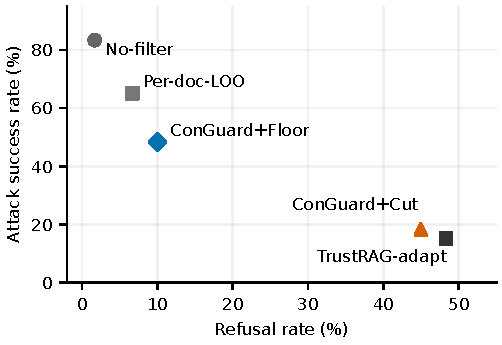
\includegraphics[width=\linewidth]{figures/tradeoff_v2.pdf}
\caption{Measured operating points on the 60-query revised attacked evaluation. Lower values on both axes are preferable; isolated points do not establish a calibrated frontier.}
\label{fig:tradeoff}
\Description{Scatter plot of attack success against refusal. No-filter has high attack success and low refusal; ConGuard plus Floor is intermediate; ConGuard plus Cut and the TrustRAG adaptation have lower attack success and higher refusal.}
\end{figure}

\subsection{Does Impact Contribute Beyond Other Features?}
\label{sec:ablation}
We distinguish removing Impact as a feature from removing its eligibility dependency entirely. ConGuard-4f uses the four features and Equation~\ref{eq:gate}; ConGuard-3f removes $I$ from the classifier but preserves that gate; ConGuard-3m removes the classifier input and uses $g_h(C)=\mathbf{1}\{m\geq2,h(C)>0\}$; and ConGuard-hgate retains $I$ as an input but uses $g_h$. The last variant isolates the gate change and is not a size-only gate. Each classifier is retrained with the same seed set, and fixed-selector outcomes are summarized in Table~\ref{tab:ablation}.

\begin{table}[t]
\caption{Strict Impact ablation on 60 attacked validation queries. The floor-preserving column fixes $(\lambda,\tau)=(0.2,0.25)$ and is identical across seeds; the hard-cut columns fix $\tau=0.5$ and report attack counts for the three training seeds.}
\label{tab:ablation}
\centering
\begin{tabular}{lcrrr}
\toprule
Variant & Floor ASR (\%) & \multicolumn{3}{c}{Hard-cut attack count / 60}\\
 & All seeds & 20260825 & 42 & 7\\
\midrule
ConGuard-4f & 66.7 & 14 & 14 & 14\\
ConGuard-3f & 66.7 & 16 & 14 & 16\\
ConGuard-3m & 66.7 & 15 & 16 & 13\\
ConGuard-hgate & 66.7 & 15 & 15 & 14\\
\bottomrule
\end{tabular}
\end{table}

All twelve variant--seed combinations have 66.7\% ASR and 6.7\% refusal under the floor-preserving selector, so the tested availability point shows no aggregate defensive gain from the Impact input or from its eligibility dependency. Equal aggregate rates do not by themselves establish that all individual predictions are identical. Under the hard-cut selector, ConGuard-4f yields 14 attacks for each seed and the other variants yield 13--16, giving mean ASRs of 25.6\% for ConGuard-3f and 24.4\% for both ConGuard-3m and ConGuard-hgate against 23.3\% for ConGuard-4f. This small, seed-dependent separation is insufficient to support a stable mechanism claim, and the seeds are repeated fits on the same queries rather than three independent test samples.

Several explanations remain compatible with these results: the other structural features may already encode the relevant distinction, eligibility changes may rarely alter selections, or the retained-context policy may block additional deletions. The complete-coalition case described in Section~\ref{sec:method} establishes one such policy restriction, though the available aggregate ablation does not quantify its contribution to the observed equality. We therefore retain Impact as an auxiliary engineering feature in the evaluated ConGuard-4f configuration rather than as an established source of improvement.

\subsection{Generation-Distribution Probes}
\label{sec:probe}
To compare graph support with generator behavior, we measure distributions with the full context and after coalition deletion. Let $y_{<t}$ be the same token prefix in both conditions, obtained from the full-context generation. For an available prefix length $T_q\leq H$, define
\begin{equation}
J_H(C)=\frac{1}{T_q}\sum_{t=1}^{T_q}\operatorname{JSD}\!\left(
P_\theta(\cdot\mid q,D,y_{<t}),
P_\theta(\cdot\mid q,D\setminus C,y_{<t})\right).
\label{eq:probe}
\end{equation}
The main maximum horizon is $H=16$, with $H=8$ and $32$ as sensitivity checks, and original token identities are retained for teacher forcing. The maximum horizon is not reached on every query: only 11 of the 63 coalition records have 16 available positions at $H=16$. For complete evidence removal the second condition is a query-only generation probe rather than the deployed selector's explicit refusal, and probing the distributions neither replaces nor modifies the deployed refusal policy.

The completed summary contains 63 coalitions from 57 queries, comprising 35 partial-evidence coalitions from 29 queries and 28 complete-evidence coalitions. For the 35 partial coalitions, the Pearson correlation of $I$ with $J_{16}$ is $0.2569$ and the Spearman correlation is $0.2835$. Table~\ref{tab:probe} gives the reported 95\% query-bootstrap interval based on 1,000 resamples; that interval includes zero and spans both negative and moderately positive associations, which is insufficient to validate a reliable generation-effect proxy.

\begin{table}[t]
\caption{Impact--probe association by removal size at $H=16$. Rows stratify the 63 coalition records by how much evidence was removed, and intervals are reported query-bootstrap intervals. The 28 complete-evidence coalitions have constant Impact, so their within-group correlation is undefined.}
\label{tab:probe}
\centering
\begin{tabular}{lrrr}
\toprule
Removal group & Coalitions & Pearson $r$ & 95\% interval\\
\midrule
Partial, all sizes & 35 & 0.257 & $[-0.135,0.565]$\\
Size 2 & 16 & $-0.323$ & $[-0.691,0.299]$\\
Size 3 & 8 & 0.502 & $[0.050,0.962]$\\
Size 4 & 11 & $-0.330$ & $[-0.779,0.286]$\\
All evidence & 28 & Undefined & ---\\
\bottomrule
\end{tabular}
\end{table}

The stratification in Table~\ref{tab:probe} shows that the pooled positive association does not persist uniformly within deletion sizes. The positive size-three estimate rests on only eight coalitions, and these exploratory subgroup intervals are not adjusted for multiple comparisons. Complete-evidence coalitions have mean probe divergence 0.4465 but all have $I=1$; including their query-only probe values closes the measurement coverage gap, though it cannot validate how Impact ranks effects within that group.

A disjoint same-size deletion control is available for 16 coalitions from 11 queries. Its mean divergence is 0.1208 against 0.1248 for coalition deletion, a paired difference of 0.0040 with reported query-bootstrap interval $[-0.0205,0.0373]$. This restricted comparison provides no clear evidence of excess influence beyond deletion size, and it does not cover large coalitions whose complement is too small to provide a disjoint control. Across all 63 coalitions, probe values at $H=8$ and $32$ correlate with $H=16$ at 0.9796 and 0.9897; that agreement concerns the horizon sensitivity of the probe rather than the validity of Impact.

Finally, $J_H$ measures a distribution change along one fixed prefix. It is neither a comparison of two freely generated trajectories nor a directional measure of factual harm, since large divergence can result from removing useful evidence and small divergence can coexist with an unchanged wrong answer. Taken together, the probe and the ablation motivate treating Impact as graph-support sensitivity whose relation to generation effects remains unvalidated.

\subsection{Clean Availability and Answer Scores}
\begin{table}[t]
\caption{Clean evaluation. Rows report refusal counts out of 300 queries per dataset and out of 900 overall, followed by answer scores on the gold-available HotpotQA evaluation subset. Gold answers are available for that subset only.}
\label{tab:clean}
\centering
\begin{tabular}{lrrr}
\toprule
Dataset & No-filter & \shortstack{ConGuard\\+ Floor} & \shortstack{ConGuard\\+ Cut}\\
\midrule
NQ & 37 & 38 & 38\\
HotpotQA & 200 & 200 & 200\\
MS MARCO & 20 & 27 & 36\\
Overall & 257 & 265 & 274\\
Overall refusal (\%) & 28.56 & 29.44 & 30.44\\
HotpotQA ESM (\%) & 11.33 & 11.33 & 11.33\\
HotpotQA token F1 & 0.1742 & 0.1742 & 0.1742\\
\bottomrule
\end{tabular}
\end{table}
Across the clean evaluation pool, ConGuard + Floor adds eight refusals and ConGuard + Cut adds seventeen (Table~\ref{tab:clean}), with the increases concentrated in MS MARCO. These aggregate increases should not be described as zero availability cost, and neither the misfilter budget nor the retention floor guarantees a fixed refusal rate.

On the 300 gold-available HotpotQA queries, all three methods have 34 exact-string matches and reported mean token F1 of 0.1742, so the available answer-quality measurement detects no degradation on this subset. It does not establish clean-answer preservation across all 900 queries. Moreover, the baseline itself refuses 200 of the 300 HotpotQA queries, and its low answer scores constrain the utility of an unchanged result; we therefore do not infer practical adequacy or statistical equivalence from equality of these aggregate scores. The absent NQ and MS MARCO gold labels prevent answer-quality conclusions on those datasets.

\subsection{Transfer Across Generators}
\begin{table}[t]
\caption{Frozen ConGuard + Floor transfer on the 60-query attacked validation pool. Rows are generator backbones and entries are percentages shown as No-filter $\rightarrow$ ConGuard + Floor. No generator-specific retuning or independent transfer test is claimed.}
\label{tab:transfer}
\centering
\begin{tabular}{lrr}
\toprule
Generator & ASR (\%) & Refusal (\%)\\
\midrule
Qwen2.5-7B & $85.0\rightarrow66.7$ & $0.0\rightarrow6.7$\\
Llama-3.1-8B & $70.0\rightarrow56.7$ & $10.0\rightarrow13.3$\\
Mistral-7B-v0.3 & $88.3\rightarrow68.3$ & $0.0\rightarrow0.0$\\
\bottomrule
\end{tabular}
\end{table}
The ASR reduction has the same direction for all three generators (Table~\ref{tab:transfer}). Llama's refusal rate, however, rises to 13.3\%, exceeding the 10\% budget used to select the Qwen operating point, so the ASR reduction transfers in direction while the availability constraint does not always transfer. The same small, development-used query pool and the similar generator scale limit broader conclusions.

\section{Discussion and Limitations}
The principal finding is a trade-off between suppressing target answers and preserving availability. The availability point achieves a larger answer-match count than no filtering in the revised evaluation, while the protection point exchanges many potential answers for refusals. Neither operating point is an unconditional recommendation, because deployment depends on how an application values wrong answers relative to unavailable ones, and the present experiment does not estimate those application-specific costs.

Several limitations bound the claim, and each suggests a concrete next step. First, semantic grouping does not distinguish collusion from legitimate repetition or establish independent evidence, and leading-excerpt truncation plus noisy NLI can miss contradictions or create spurious groups. Singletons are not scored, and the floor-preserving selector cannot remove an all-evidence coalition. Separating grouping from non-grouping under a matched selector would isolate what the coalition abstraction itself contributes. Second, all attacked results use a five-passage retrieval setting and one targeted synthetic attack construction, and the available family-level records do not establish separate, reproducible corpus snapshots. We therefore make no validated family-generalization or adversarial-training claim; re-running the frozen configuration on independent corpus snapshots would test that generalization directly.

Third, the revised attacked pool was used during development and the generator-transfer results reuse validation queries, so no attacked independent confirmation is reported here. Fourth, TrustRAG-adapt is a project adaptation without a matched-refusal operating curve, and clean-answer labels cover only one dataset; scanning the selector threshold to refusal-match that baseline would replace the present incomparability with a direct comparison. Fifth, the newest ablation and probe findings are available as aggregate records whose per-query traces are absent from the accompanying archive, which limits independent checks of intervals and per-query transitions, and older traces from a different snapshot cannot fill that gap. Finally, timing summaries cover warm batches, and end-to-end online latency was not measured.

For autonomous agents, the contribution concerns filtering external evidence before it is consumed. It does not demonstrate safer tool use or improved completion of agent tasks, and a document coalition should not be read as a multiagent interaction merely because the filter is applicable upstream of an agent. These boundaries separate the implemented mechanism from applications that remain unevaluated.

\section{Conclusion}
We introduced RAG-ConGuard, an inference-time coalition-level evidence filter with two explicit context-selection policies. In the examined targeted-poisoning setting, it reduces attack success relative to no filtering while exposing a substantial safety--availability trade-off, and the available TrustRAG comparison does not establish superiority. The ablations and probes do not establish an Impact benefit at the availability point or validate it as a proxy for generation effects, so we retain Impact as an auxiliary graph-support feature. Taken together, the contribution is coalition-level evidence filtering and its measured operating trade-offs, offered as a step toward evidence-intake control for knowledge-grounded agents; the findings remain exploratory, and closed-loop evaluation on agent tasks remains open.

\paragraph{AI assistance.}
Use of ChatGPT, Codex, and Claude is disclosed in the supplement.

\balance
\bibliographystyle{ACM-Reference-Format}
\bibliography{references}
\end{document}
